\chapter{Background}\label{C:us}

%What background is there into the research domain

%Web-scraping background and concepts

%Social media personality analysis

%Social media behaviour analysis, showing that social media actions correspond to individuals real-life actions to some respect

%Classification and dynamic access-driven policies, could these potentially be applied to social media

%Quantifying reputation on social media - what this means. Examples of systems that attempt to quantify reputation on social media, through the use of APIs and how a system I build could extend upon these. 

This section covers the background research performed for the project, and works related to the project. Also discussed are the contributions to the research domain, with points of different to these related works.

% I also discuss how I was able to contribute to the research domain, with points of difference to these works. 

\section{Social Media}

Social Networking Sites (SNS) have achieved massive adoption and user numbers since their inception. SNS describes any web site that enables users to create public profiles and form relationships with others. The SNS market has largely stabilised, with Facebook achieving market dominance. When deciding which sites to fetch data from, research was conducted into the most popular SNS, and features that could be applied into some reputation score. In order to fetch useful information, various social media sites were investigated in the context of gathering reputation data, and seeing what could be selected.

% In order to fetch useful information, I looked at the various social media sites in the context of gathering reputation data, and seeing what could be selected. 


%Insert diagram of the social networking market share. 

%Social Media Sites (SNS) 

%A background to social media. What defines a social media site. 

%What are social media sites

%What sites did I scrape, what was I able to do

%Web scraping was the technique used, discuss this next.

%Until now, the reasoning behind my social media selection has been largely neglected. In order to gather useful data, I looked at the various social media sites in the context of gathering reputation data, and seeing what could be fetched. %Add to this. Not very good currently... 


\begin{itemize}

\item Facebook \cite{facebook_site}: Publicly available information on Facebook includes data such as a user's Likes, Posts to Walls, and Friend networks. 
\item LinkedIn \cite{linkedin_site}: The primary business social network on which professionals can display information pertaining to their career and skills. Reputation data is fairly concrete - endorsements, skills, groups, and recommendations. 
\item Twitter \cite{twitter_site}: A SNS allowing posts of up to 140 characters. Information available includes number of followers, number of profiles the person is following, number of posts, and post data itself. Post data includes retweet and favourite count, the content itself, as well as the people who retweeted the tweet itself. 
\item Google+ \cite{google_site}: Similar to Facebook in style, and holds a large user base, but with much lower daily use than Facebook.
\item Slashdot \cite{slashdot_site}: A social media and news network targeted at a 'geek' audience. Slashdot is one of few social media sites that uses a positive/negative rating system on posts. This inbuilt reputation system could be interesting to look at further, when porting data between social media platforms. It is also unique from the standpoint of identifying 'trolls' - for which the website is widely known. 
\end{itemize}

This basic feature analysis was the foundation for data exploration on the social media sites scraped. As the project's primary aim was to demonstrate the feasibility of web-scraping as a means for fetching such information, research was conducted on web-scraping as a technology. 

\section{Web-Scraping}

% Web-scraping or \textit{screen scraping} refers to the practice of downloading web pages directly through HTTP requests, and parsing this unstructured data into something useful. It is a wel-understood data-gathering technique, and there are existing architectures and frameworks to help facilitate this. Anything online that is accessible through a browser can be scraped. 

Web-scraping or \textit{screen scraping} refers to the practice of downloading web pages directly through HTTP requests, and parsing this unstructured data into something useful. It is a well-understood data-gathering technique, and there are existing architectures and frameworks to help facilitate this.  Anything online that is accessible through a browser can be scraped. Hartley gives a light introduction to the concepts and strengths of web-scraping \cite{no_api_for_me}. Web-scraping is largely used as an alternative to traditional website APIs, where these may not exist, or face a lack of support or development. Applications using web-APIs which frequently change could also benefit from switching to a web-scraping alternative. The advantage of web-scraping is that it provides direct access to the content of a website. While a site's API may not allow access to information that is quite clear from the front end, web-scraping will inherently provide this. Also, some sites do not monitor their API 
status 
as carefully as the actual front-end access. Maintaining availability to the core site is of higher business priority than developer APIs, and this is consistently reflected in respective levels of support. 

The primary limitation of web-scrapers is that major user interface changes will likely result in a broken scraper. In general site's structures do not change frequently enough for this to be a major issue. The typical argument however is that a site's structure can, without any warning, change at any time. This is an unavoidable issue when considering developing a scraper, and as such the regularity of user interface changes on a website should be considered when deciding between using an API or a scraper. In general it is more sensible to inspect a site's API for applicability before constructing a web-scraper. As an example; Facebook was ruled out as a social option in this project due to its regular user interface updates. 

However these interface change limitations can also be applied to modern social media APIs. Past projects fetching data from Facebook have had difficulty maintaining applications due to its too-often changed API \cite{kosinski2013private}. In the course of this project, Twitter's API changed such that the possibility of fetching required data through this interface was rendered infeasible. When considering scraping data, legal and privacy considerations must also be applied.

%Limitations of scrapers
%Although web-scrapers tend to break when user interfaces change, in general sites structures do not change frequently enough for this to be a major issue. However they can, without any warning, change at any time which limits web-scraping as a technology. Keep in mind that most websites do not change so frequently as for this to be an issue, although it did rule out Facebook as a candidate for my project. 

%A counter to the limitations of web-scrapers is the frequency of API changes on modern social media sites. Past projects fetching data from Facebook have failed due to its too-often changed API \cite{}. In the course of this project, Twitter's API changed such that the possibility of fetching required data through this interface was rendered infeasible. When considering scraping data, legal and privacy considerations must also be applied.

%Look at some applications of web-scraping.

%Web scraping vs APIs?

\subsection{Legal and Privacy Issues}

Companies such as Google and Facebook are widely known to use web-scraping on SNS and other sites for the purposes of web-indexing and advertising \cite{no_api_for_me}. Despite this, other entities attempting to commercialise such aggregated data have been met with threats of hostile law action. Pete Warden discusses how his data-mining experiences on Facebook nearly resulted in legal action \cite{facebook_sued}. In these cases though, data-mining was intended to be used for commercial purposes. 

As an academic project, fears of legal retaliation are much lower. However strategies were enforced in order to stay within the terms of service of social sites. By never signing into the SNS that I retrieve data from, I inherently do not agree to the user terms of service\footnote{https://twitter.com/tos}. I also followed general positive web-scraping practices where possible, in order to limit possible negative effects of my scrapers upon these sites. Examples include attempting to adhere to a sites robots.txt, and the placement of reasonable pauses between requests to reduce server burden. 

\section{Inferring Information from Social Media}

The following sections examine research conducted into what information has already been investigated on social media. In particular, private personality traits that are inferable from publicly available data are discussed, as well as how sentiment analysis of SNS can predict unexpected variables. 

% I now examine research conducted into what information has already been investigated on social media. In particular I discuss what private personality traits are inferable from publicly available data, as well as how sentiment analysis of SNS can predict unexpected variables.
%In particular what private personality traits can be inferred from publicly-available data, as well as 

%Discuss the core challenges of web scraping in a social media setting

\subsection{Personality from Social Media}

Studies have investigated how private details about personality traits can be inferred through behavioural analysis of individuals on social media \cite{adali2012predicting,adali2012actions,bachrach2012personality,golbeck2011predicting,golbeck2011computing,golbeck2011,golbeck2011experimental}. Golbeck et al. demonstrate that real life personality traits may be predicted by looking at past behavioural patterns on Twitter with high accuracy \cite{golbeck2011predicting}. Using the publicly-available figures of followers, following and posts the authors were able to classify individuals into different Big Five personality types \cite{de2000big}. This was verified against a 44-question personality test for 71 individuals, with accuracy of around 80\%. In further papers these authors were also able to make conclusions on political preference, as well as extend their work onto Facebook and tagging behaviour \cite{golbeck2011computing,golbeck2011,golbeck2011experimental}. Adali et al. \cite{adali2012predicting,
adali2012actions} extend this work further by predicting personality and relationship information on Facebook.
%Sentiment-based analysis of tweets has also been studied, analysing the use of emoticons on Twitter.
%Studies have shown how private details about personality traits can be inferred by behavioural analysis of individuals on social media. These studies have taken both a behavioural-based and textual sentiment-analysis approach to determine personality. Studies showed that real life personality traits can be predicted by looking at past behavioural patterns on Twitter, with high accuracy \cite{}. Using publicly-available information on Twitter pages, the authors were able to classify individuals into different Big-Five personality types \cite{}. This was verified against a 44-question personality test for 71 individuals, with accuracy of around 80\%. Further research has been performed, looking at how Facebook behavioural patterns relate to personality type by asking questions on the MyPersonality Facebook app. Behavioural data was then gathered from the test subject's Facebook profiles, to check for correlations. Textual sentiment-analysis approaches have also been taken in order to determine personality 
% type 
%from social media profiles. Sentiment-based analysis of tweets has also been studied, analysing the use of emoticons on Twitter \cite{kewalramanisentiment}.

While these studies showed how private personality details can be inferred from publicly-available data, they were made using applications which had to be given express permissions to access this data. In other words, although the conclusions drawn from these papers was that massive data-mining could be undertaken on these profiles as all the data is publicly available, they never used an approach that demonstrated the true feasibility of this. Clearly as social media site APIs are properly locked-down and require authorisation of the relevant users to retrieve data\footnote{https://developers.facebook.com/docs/reference/apis/}, a web-scraping approach must be used. Such an approach allows applications to only require the same permissions as any human being accessing the same page, whilst also allowing the same data to be downloaded and aggregated.

A potential weakness in these studies is that personality on SNS may not translate well into actual personality. Although this may seem like a logical conclusion (consider Trolls, shallow internet relationships), studies have shown it to be false. Quercia et. al. demonstrated how popular Facebook users in fact maintain meaningful relationships with their hundreds of friends, and not the superficial ones we may expect \cite{quercia2012personality}. Again the Big Five personality model was used, and verified against popular Facebook users who used the MyPersonality app. Back et al. \cite{back2010facebook} demonstrated how Facebook profiles in fact are reflective of actual personality, and not a self-idealisation . This study used manual inspection of profiles to make first impressions of individuals, which were compared against results from a Big Five personality test. Making similar predictions with computers would be an interesting and difficult challenge. 

\subsection{Sentiment and Temporal Information from Social Media}

It is also possible to take sentiment and temporal-related information from social sites as a whole, and use trending information to make accurate predictions about seemingly unlinked occurrences. Bollen et al. \cite{bollen2011twitter} demonstrated that the 'mood' of Twitter can be used as a predictor of the U.S. stock market. The authors argue that Twitter mood is an accurate predictor of the public's mood state in general, which affects human decision-making and as such financial decisions. By taking historical Twitter data and calculating mood values using a classifier, the authors showed that Twitter was an accurate predictor of the U.S. stockmarket.

In a similar temporal approach to social BigData analysis, Ginsberg et al. \cite{ginsberg2008detecting} investigate the detection of influenza epidemics using Google search query data. By analysing the relative frequency of certain queries implying health information-seeking online, early prediction and detection of epidemics may be possible. These examples demonstrate that information that may be thought of as separate can be determined from the wealth of information on social media.

%Talk about research conducted into social media, with respect to temporal analysis and predicting stock markets, etc.

%Various temporal-clustering and sentiment based analysis studies have been conducted on social media. Bollen et al \cite{} demonstrated that the 'mood' of Twitter can determine the U.S. stock market. 
\section{Quantifying Reputation on Social Media}

% The above studies demonstrate how private personality and public 

Although the above studies investigate the concept of personality and how we can quantify this using social media, they did not expressly address the concept of reputation. Therefore we should discuss what reputation explicitly means on social media, and how sites currently help express user reputation. 

Some sites explicitly reference user reputation, a system commonly utilised on social forums. Stack Overflow \cite{stackoverflow_site} is a question and answer site where users are able to post code-related programming problems. It has been identified that sites such as Stack Overflow are largely dependant on the contributions of a small number of expert users, who provide a significant proportion of useful answers \cite{movshovitzanalysis}. As such, identifying users who have the potential to become strong contributors is of significant importance to the success of the website.

\begin{table}[h!]
\begin{center}
\begin{tabular}{l|r}
 Action & Reputation Change\\ \hline
 Answer is voted up & +10 \\
 Question is voted up & +5 \\
 Answer is accepted & +15 (+2 to acceptor) \\
 Question is voted down & -2 \\
 Answer is voted down & -2 (-1 to voter) \\
 Experienced Stack Exchange user & onetime + 100 \\
 Accepted answer to bounty & +bounty \\
 Offer bounty to question & -bounty \\ 
\end{tabular}
%Actions and Corresponding Reputation Change on Stack Overflow \cite{movshovitzanalysis}
\end{center}
\caption{Actions and Corresponding Reputation Change on Stack Overflow \cite{movshovitzanalysis}}
\label{tab:STACK}
\end{table}

%Actions and Corresponding Reputation Change on Stack Overflow \cite{movshovitzanalysis}\\

%\caption{Actions and Reputation Change on Stack Overflow\cite{movshovitzanalysis}}\\

Table \ref{tab:STACK} defines the actions and corresponding reputation changes users may take on Stack Overflow. Reputation in this context is entirely derivative of the actions and effectiveness of answers provided by users. Within Stack Overflow, a high user reputation score could be considered a measure of expertise.

The online forum SlashDot \cite{slashdot_site} is another social site where user action affects reputation. Slashdot was created in 1997 as a 'news for nerds' message board \cite{josang2007survey}. As member numbers grew rapidly, spam and poor posts became an issue, resulting in the introduction of a moderation system.A two tier moderation system now exists, with \textit{M1} administrating comments on articles, and \textit{M2} moderating the \textit{M1} moderators. User reputation information is recorded using \textit{Karma} for logged in users as a reputation metric. Each logged in user maintains a \textit{Karma} score from one of six discrete values: \textit{Terrible, Bad, Neutral, Positive, Good, Excellent}. Positive moderation feedback to a user's comment will result in an increase in Karma. The opposite applies for negative moderation. Comments on SlashDot are ranked from [-1,5]. If a user with high Karma created a comment, this will have a higher starting rank. To reduce spam, users can then filter 
comments based on minimum rank. For example if a user wished only to see the best comments, they could set the filter value to 5. 

The SlashDot reputation system is an example of effective spam filtering through the use of a reputation system in conjunction with moderation. The use of reputation in this context greatly reduces the moderation community effort to maintain the website. 

%Each of these users maintains a \textit{Karma} score in the range [-1,5]

%\noindent Reputation in this context is entirely derivative of the actions of users. In the context of Stack Overflow, a high user reputation score could be considered as a measure of expertise.

%Give examples of some other sites. Reddit and Slashdot are two classic examples that contain some concept of reputation. 

\section{Reputation Metrics Elsewhere}

Reputation systems have also had considerable success on trading applications such as eBay and TradeMe. Resnick et al. \cite{resnick2000reputation,resnick2002trust} looked at the success of eBay's reputation system and identified the following three properties that a reputation system must enforce in order to add value to such a site. 

\begin{itemize}
 \item Entities are long-lived, so that there is an expectation for future interaction. This generates a \textit{shadow of the future}, and provides incentive for users to behave with integrity in the short term, such that future interactions will not be impacted by a poor reputation. 
 \item Feedback about current actions is captured and visible to others. This ensures that users are able to pay attention to their own and other's reputations, when interacting with other community members. 
 \item Feedback from the past guides current decisions: people must pay attention to reputations for them to be valuable. 
\end{itemize}

This impacts the undertaken research as it guides the creation of reputation policies; reputation data I gather should conform to these concepts. Resnick's paper also identified weaknesses within current reputation systems online. There are three weaknesses present within current reputation systems which automated policies can help address. 

\begin{itemize}
 \item Fears of retaliation - users not posting negative scores due to fear of unsolicited reciprocation.
 \item People not bothering to place feedback - if no incentive exists for users to place feedback, they may not see the value of doing so.
 \item The assurance of honest feedback - for the above two reasons, reputations may be skewed and not reflective of reality.
\end{itemize}

An automated reputation system using policies to turn reputation into access or action rights solves many of these issues instantly. There is no area in which retaliation can occur, feedback is never explicitly placed, and policies treating all users equally will assure honest feedback.

\section{Related Work}

The following sections review and discuss a number of related works. The Generalised Recommendation Architecture and an OpenSocial access framework are covered in the context of access control solutions using reputation attributes as keys. Then the social media focused reputation system Klout is discussed.

% I will now discuss some systems which consider reputation data and apply it to access-control and service selection policies online. Firstly I examine the Generalise Recommendation Architecture and an OpenSocial access framework, in the context of access control solutions using reputation attributes as keys. Then the social-media based reputation system Klout will be discussed. 

%Finally, the social-media based reputation system Klout will be discussed. 

%I will now discuss some systems which consider reputation data and apply is to access-control policies online. This is only one potential application of the generation of reputation metrics, but such applications add considerable value from an administrative point of view when compared to, say, traditional Virtual Organisation (VO) access policies on Grid systems. Having looked at GRAft and an Open Social application, I move on to more social-media focused systems such as Klout.
% 
% \subsection{Service Oriented Computing}
% 
% Service Oriented Computing (SOC) is a computing paradigm in which software applications are constructed based upon independent component services with standardised interfaces \cite{tsai2006introduction}. An emerging issue with this concept is how to select appropriate services based upon the application's needs. In the traditional model, service providers publish descriptions of their services in the service registry that is used by service clients to discover and select services. Najafi et al. identity four issues with this model \cite{najafi2012web}.
% 
% \begin{itemize}
%  \item Service descriptions provided by the service provider may not be accurate or trusted
%  \item Service descriptions generally do not capture specific performance requirements for different client's needs, in different contexts
%  \item Less well-known services do not get an opportunity to show their features
%  \item Service features vary with different measures, and are obtained under different situations, thus cannot be fairly compared. 
% \end{itemize}
% 
% Proposed solutions have suggested approaches such as promoting competition between webservices, using an independent entity to evaluate the different web services against given criteria. %More discussion... Can't think right now!
% 
% The Generalised Recommendation Architecture (GRAft) is an example of such a framework that could store such reputation data.

%\subsection{Virtual Organisations}
%I will provide some background on Virtual Organisations, and discuss their limitations in order to validate the requirement for improved access control policies on Grid Systems. A VO running on the Grid allows users to access resources that are physically distributed in different locations \cite{}. Most VO frameworks support the concept of inter-institutional trust. But any user who wishes to access these resources must have an identity that is trusted by all service points and obtain permission from the authorisation server. This access model is inflexible when adapting to scientific collaborations which are often flexible and dynamic. VO administrative features lack the ability to easily describe fairly casual or temporary trust agreements between research groups \cite{}.

%To achieve data security in a VO, user authentication is based upon a very tightly controlled trust relationship between resource providers and users. Every user must have an identity mapped to multiple IDs, in order to authenticate with the complex procedure, requesting access to a particular resource. These authorisation procedures on many popular VO access models result in large administrative burdens. I would argue that such a burden will become more and more infeasible in e-Science, given the increasingly large communities of researchers, educators and students \cite{}. Such an access control model would never be feasible on the social media. 

%There are potential security vulnerabilities exposed when working with an access system that does not reflect the needs of users. Security relies on organisations following the prescribed protocols, and that these protocols are not overly onerous on individuals. If this is not the case. users may create workarounds, resulting in security being compromised. This is not inconceivable in VO systems. For example, blanket access may be prescribed to organisations where this may not be appropriate. 

%It's also worthwhile considering the semantic meaning of relationships online or on a scientific Grid when designing an access mechanism to suit these relationships. These relationships are ad hoc, flexible and changing. The VO model of access is none of these. We should consider that in a VO, trust relationships are stored in one central point, whereas trust information in reality is stored at the level of individuals. It thus makes more semantic sense to move trust information onto the nodes of a system. The following access control models, that use reputation information as key drivers for access decisions, are examples that better reflect these requirements.

\subsection{Generalised Recommendation Architecture}

The Generalised Recommendation Architecture (GRAft) \cite{graft_paper} is a distributed architecture that supports the collection and storage of reputation information for entities, whether these be individual users or systems. It uses the OpenID \footnote{http://openid.net/} infrastructure in order to maintain long-term identity for users. To ensure validity of reputation data, information within GRAft is duplicated over the nodes (using a distributed hash-table) which comprise the network. 

Entities within GRAft are uniquely identified using their OpenID. The system is able to maintain a history of the entities actions, including recommendation and transactional history. In this fashion, entity \textit{profiles} are established, with recommendation data being pulled from multiple sources, each source acting as a \textit{source node}.

%Add more to this

%Change this to he forum example. More relevant to my studies than the example pictured here. 

Although GRAft is not a system currently used in industry, the authors discuss how it could be applied in practice. The domain of a scientific wiki is one such example. This wiki consists of scientific articles, which can be read and edited by members. Using a two-tier access policy defined in Figure \ref{fig:GRAFT}, read access to a page was is given by co-authorship. Users who had previously worked with the owner have a 1st-degree relationship; those who have worked with a person in the set of 1st-degree owners are 2nd degree owners, and so on. Once the user is granted access depending on this degree of co-authorship, editing rights are calculated by the users Hirsch-Index (H-Index) \cite{hirsch2005index}. Another policy is then responsible for assigning editing permissions based on this value. This example demonstrates how access rights can be automatically granted for all users who fulfil requirements defined by the page owner. The group is never explicitly defined in terms of users; and as the author 
begins work with others, they can be automatically granted access to resources. This flexible policy comes closer to reflecting ad-hoc and informal scientific collaborative interactions, and is based on trust information that comes closer to real-life reputation. GRAft as a distributed reputation storage system has the potential for storage of reputation data for many different applications. By implementing reputation policies for storage within GRAft, this project provides a further case study example for this system.

% My proposed solution extends and borrows concepts from these related reputation systems. GRAft as a distributed reputation storage system has the potential for storage of reputation data for many different applications. By implementing reputation policies for storage within GRAft, I essentially create source nodes as a further case study example for this system.

% Whilst Klout provides interesting reputation insight into a users profile, it is limited in that only your own profile reputation data can be viewable immediately. To view friend's profiles, they must sign into Klout themselves. It is impossible to view the Klout scores for strangers. As such this system is only purposed for competition among friends, and little else. 
% Figure \ref{fig:GRAFT}

\begin{center}
\begin{figure}[h!]
\begin{verbatim}
 $rb->logicalAnd(
  $rb['hindex']->greaterThanOrEqualTo(1),
  $rb->logicalAnd(
    $rb['degree']->greaterThanOrEqualTo(0),
    $rb['degree']->lessThanOrEqualTo(3)
   )
 )
\end{verbatim}
\caption{GRAft reputation based access policy example}
\label{fig:GRAFT}
\end{figure}
\end{center}


\subsection{Open Social}
%How can GRAft be used and what value does it add.

Zhang et al. \cite{zhang2012open} proposed an Open Social\footnote{http://opensocial.org/} based group access control framework. Open Social is a framework for deploying cloud-based social applications. It was used in this context as it provides an API useful for retrieving social connection data. It also supports OAuth\footnote{http://oauth.net/}, a protocol that allows users to grant third-party access to their protected resources.

The social trust scheme proposed in this paper consists of a multi-tenancy access control model, which can be applied to a scientific team-management scenario. Firstly the authors consider how trust in this context is a complex human-to-human relationship, developed through scientific collaboration. The authors argue that information about such relationships can be captured through data embedded on Online Social Networking (OSN) sites. This enables friend-of-a-friend trust to be computed, enabling transitive data as also seen in GRAft(which proposed using degree of co-authorship as a trust attribute). Whilst this system is useful for access control schemes, there was little discussion relating to other potential applications of its reputation schemes. By creating a more generic social media scraper, this project increases the possible avenues for utilisation of this data.

%  Whilst the Open Social based reputation system is useful for access control schemes, there was little discussion relating to other potential applications of its reputation schemes. As such it is of arguably less value than a more generic system such as GRAft. 

%How do social media sites control access
%How effective have social media sites been at controlling access, and how well do users feel that their information is safe?

\subsection{Klout}

Klout \cite{klout_site} is a social media reputation system that generates an \textit{impact score} out of 100, based on how influential you are on various social media sites. In order to generate a Klout score, users sign in to Klout using OAuth to connect to their social media site of choice. Klout then interacts with these sites' APIs to fetch the relevant data. Figure \ref{fig:KLOUT} shows Klout's dashboard page, which breaks down a user's reputation score. This site is useful as it both demonstrates how such information can be used to generate influence information, as well as how such a system can become popular. I extend this system by using the alternative approach of web-scraping. By doing so, users would be able to look at the reputation data of other users, as well as themselves. 

\begin{figure}[h!]
\centering
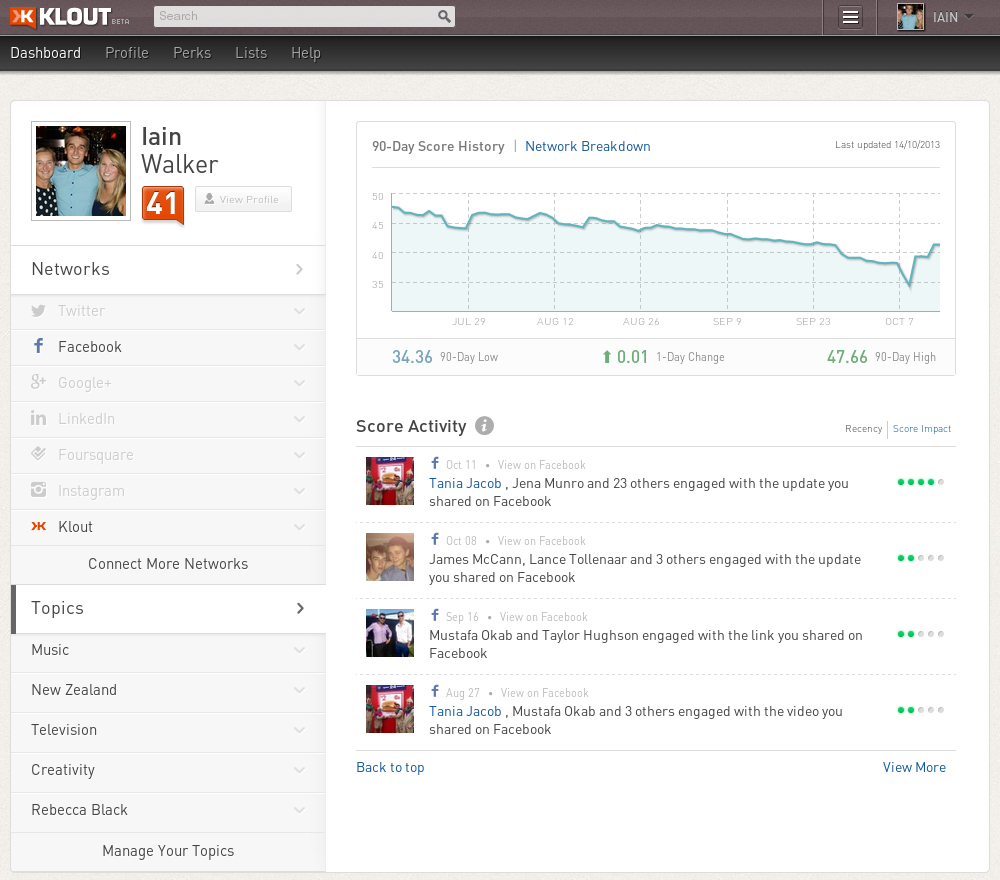
\includegraphics[width=0.7\textwidth]{Images/klout.png}
\caption{Klout impact score}
\label{fig:KLOUT}
\end{figure}

% \subsection{Discussion}

% My proposed solution extends and borrows concepts from these related reputation systems. GRAft as a distributed reputation storage system has the potential for storage of reputation data for many different applications. By implementing reputation policies for storage within GRAft, I essentially create source nodes as a further case study example for this system. Whilst the Open Social based reputation system is useful for access control schemes, there was little discussion relating to other potential applications of its reputation schemes. As such it is of arguably less value than a more generic system such as GRAft. 

% Whilst Klout provides interesting reputation insight into a users profile, it is limited in that only your own profile reputation data can be viewable immediately. To view friend's profiles, they must sign into Klout themselves. It is impossible to view the Klout scores for strangers. As such this system is only purposed for competition among friends, and little else. 

%Add more reflection and discussion about the related systems, and discuss why a new solution needs to be developed. Otherwise, why don't we just tsick with the current system lol

%Discuss how my system is different from these related systems, and how it adds value. 

%Graft system

%Klout

%How did my research relate to the existing works reviewed, and to what extent my work can be distinguished from them. 